\begin{figure*}[!tb]
  % 
\includegraphics[width=\textwidth]{Colm/failure_distribution.pdf}
  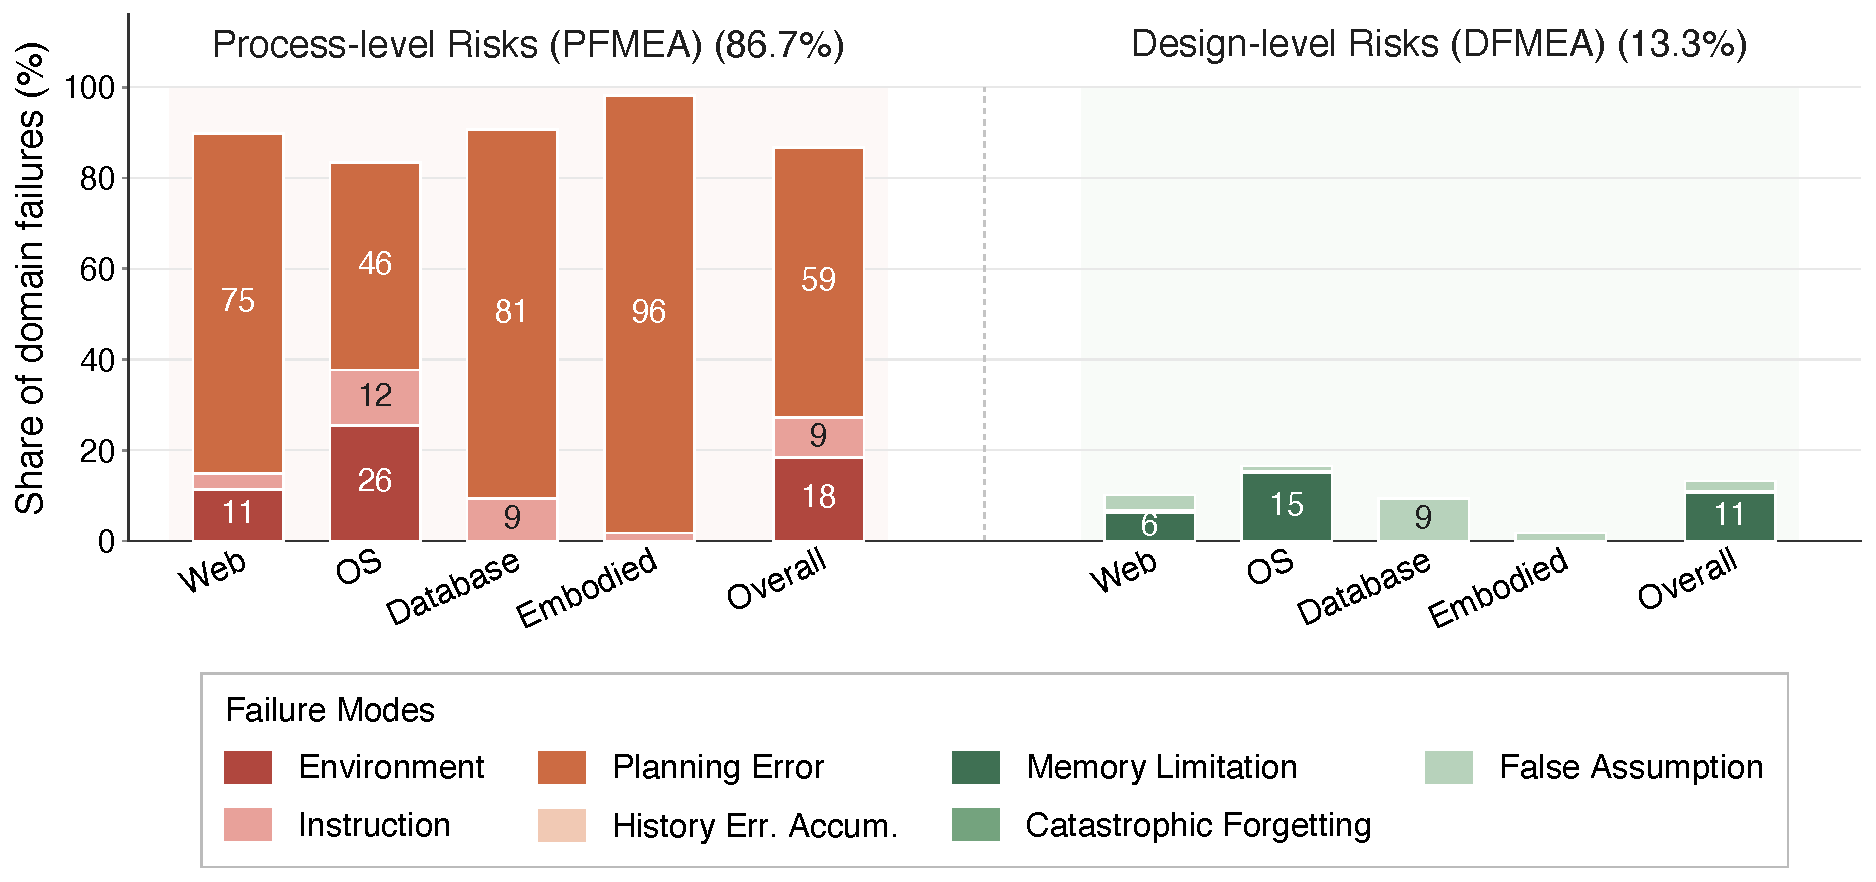
\includegraphics[width=\textwidth]{failure_distribution.pdf}
    \centering
  % \caption{\textit{Distribution of failure modes across domains and models on \totalfailures{} failure trajectories.} 
  % Bars are grouped into three categories: Planning \& Reasoning Errors (59.5\%), 
  % Environment \& Instruction Failures (29.0\%), and Memory Limitation (11.5\%).
  % Within each category, bars show per-domain/model breakdowns stacked by failure sub-type.\jessica{change caption}}
  % \label{fig:failure_distribution}
  \caption{\textit{Distribution of failure modes across four task domains on 3100+ trajectories.}
  Bars show the proportion of each failure type relative to the total failed traces within each domain.
  Failures are grouped into Process-level Risks (PFMEA) (environment, instruction, planning errors, and history error accumulation) and Design-level Risks (DFMEA) (memory limitation, catastrophic forgetting, and false assumptions). More details are provided in Section~\ref{sec:5}.}
  \label{fig:failure_distribution}
\end{figure*}